\documentclass{article}

% Language setting
% Replace `english' with e.g. `spanish' to change the document language
\usepackage[english]{babel}
\usepackage{float}
\usepackage{multicol}

% Set page size and margins
% Replace `letterpaper' with `a4paper' for UK/EU standard size
\usepackage[letterpaper,top=2cm,bottom=2cm,left=3cm,right=3cm,marginparwidth=1.75cm]{geometry}

% Useful packages
\usepackage{amsmath}
\usepackage{graphicx}
\usepackage{wrapfig}
\usepackage{svg}

\usepackage[colorlinks=true, allcolors=blue]{hyperref}

\title{HarMMMLonizer}
\author{Lelio Casale, Marco Furio Colombo, Marco Muraro, Matteo Pettenò}
\date{102827, 10537094, 10866647, 10868930}
\begin{document}
\maketitle

\begin{abstract}
Among several definitions, music is a category of perception as it involves cognitive processes. Harmony is one of the building blocks of Western Music, along with melody. Indeed, exploiting the vertical dimension of music, the musician can manage the mood of the song and convey specific emotions to the listener.
Harmonizer is one of the most used audio effects within the music professionals community. The project presented in the following paper is focused on the implementation of such a digital signal processor through SuperCollider, including a graphical user interface to control the available parameters. Moreover, the software provides the user with an additional component devoted to delay effect to be applied individually on pitched voices generated by the harmonizer itself. Different feedback settings can be chosen by the musician.

\end{abstract}

\section{Introduction}

\subsection{Basic Principles of the Harmonizer}
The main structure of an harmonizer is based on many voices, usually three or four. Each voice is the pitch-shifted version of the input of a certain amount of semitones. Pitch shifting means multiplying every frequency of the input by the $n-th$ power (n is the number of semitones we want to shift the signal of) of a factor that represents the ratio between a note and the note that is one semitone below, which is the twelfth root of two  (around $1.05946$). As an example, if we want to obtain a voice shifted by a third (4 semitones), we have to multiply each input frequency by $(1.05946)^4$.
Pitch shifting differs from frequency shifting: in frequency shifting a certain amount of Hertz is added to every frequency, with the result that the ratios between the fundamental frequencies are not maintained. Instead, in pitch shifting, the ratio between fundamental frequencies of the input is guaranteed by the fact that every frequency is multiplied by the same quantity.
Pitch shifting is recommended for small intervals, usually maximum an octave or a little bit more, for bigger intervals we may introduce a distortion that affects the quality of the shifted signal. This is the reason why usually in a harmonizer we’re allowed to shift the input signal by two octaves above (which means a factor of 4) and below (which means a factor of 0.25).
Other features can be added to a harmonizer, also depending on the needs of the artist and the musical genre. Usually a gain knob is provided to the user, to adjust the volume of each voice. This choice is made both for an artistic reason and for a psychoacoustic reason. In fact, the human ear is not sensitive to all frequencies in the same way: sounds with a mid-high fundamental frequency (100 Hz to 4000 Hz) tend to be perceived as louder. So if we want to hear a low and mid-high frequency pitch shifted voice of the harmonizer at the same level, we need to set the gain of the low voice higher than the gain of the mid-high voice.
Also a delay control and a pan control for each voice are usually provided to the user, the first one to add some delay effects, and the second one to have fully under control the spatial stereo direction of each voice.

\begin{figure}[H]
\centering
 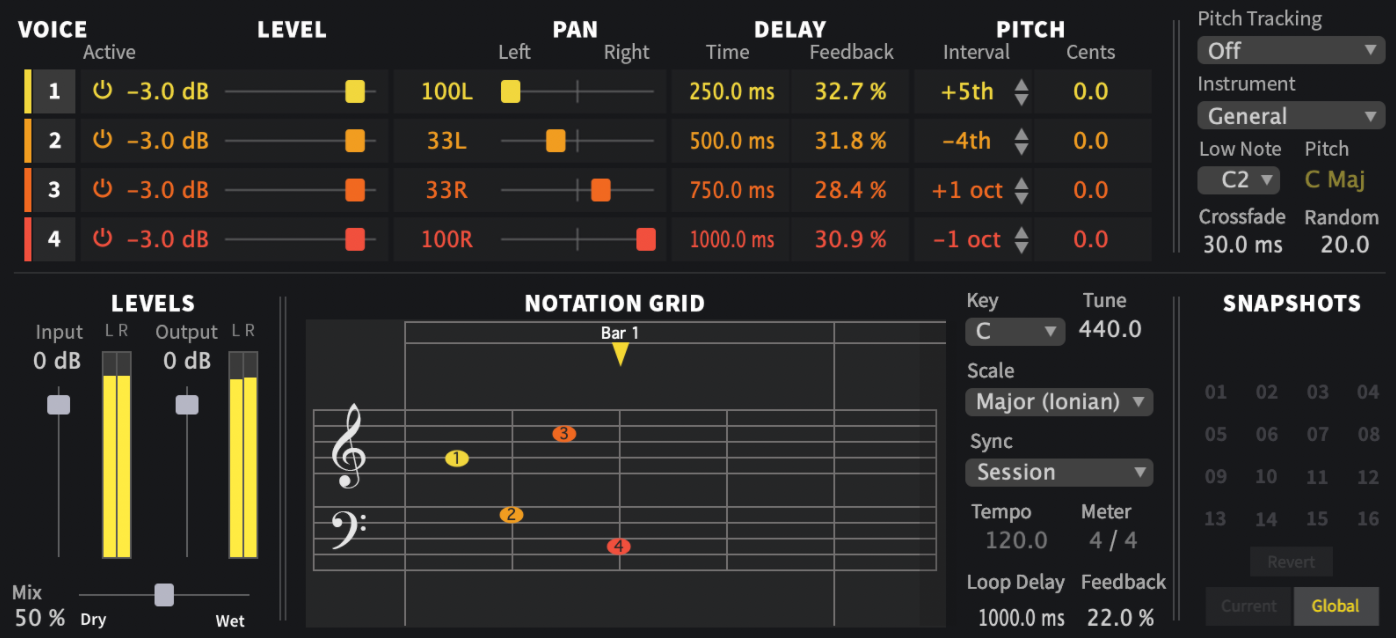
\includegraphics[width=0.75\textwidth]{quadravox.png}
  \caption{An example of a four voices digital harmonizer - Quadravox by Eventide.}
\end{figure}

\subsection{Purposes}

The project aims to develop a real-time harmonizer, i.e. an audio-based software which provides the user with the possibility of creating a two or more notes harmony. The application was implemented through SuperCollider, a powerful engine for sound synthesis and algorithmic music composition which offers a sound-based, real-time and object-oriented programming language.
 \begin{itemize}
  \item Implementation of a pitch-shifter block which takes a signal as an input and returns the shifted version as an output. The software must support a maximum of three pitch-shifted voices.
  \item Implementation of a delay line block which accomplishes delay effect on the pitch-shifted signal, with the possibility of different feedback configurations. Each pitch-shifted voice is processed individually within this block.
  \item Implementation of a Mixer component so that the user can control the master volume and stereo pan of the final output.
  \item Development of a Graphical User Interface (GUI) in order to provide the user with the possibility of controlling the available parameters, such as Pitch Ratio, Delay Time and Feedback Mode.
\end{itemize}
 

\section{Implementation}
\subsection{Software Architecture}
The architecture of the whole software consists of two main components: the \textbf{audio processing block}, responsible for signal processing, and the \textbf{graphical user interface (GUI)} which implements the graphical component of the software itself.
\\The \textbf{audio processor} in turn is composed of three functional blocks which are the Harmonizer, a Delay Line and a Mixer. These blocks were implemented through SuperCollider language as SynthDefs (Synthesizer Definitions) with specific available arguments with respect to what parameters the musician needs to control through the GUI. An additional block was implemented with the purpose of collecting the input signal coming from the sound card and writing it on a specific bus so that the implemented synthesizers can read it and compute processing operations on the signal.
\\The \textbf{graphical user interface} shows three main sections, one for each harmonized voice so that the user can select the desired values for the parameters of the harmonizer and delay line. Furthermore, a mixer section is made available in order to allow the musician to control master volume of the final output and dry/wet balance between the clean input signal and harmonized voices.
\\As the software is designed, the server allocates the following mono audio buses:

 \begin{itemize}
  \item \textbf{\textit{$\sim$inputAudioBus}} collects the input audio signal coming from the sound card.
  \item \textbf{\textit{$\sim$pitchShiftedVoiceBuses}} is an array of three audio buses representing the pitched voices generated by the harmonizer.
  \item \textbf{\textit{$\sim$delayedVoiceBuses}} is an array of three audio buses representing the delayed voices of the harmony.
\end{itemize}
In addition to this, three arrays of one channel control buses are used with the purpose of sending parameters values related to each single voice from the GUI to the different synthesizers instantiated on the server:

 \begin{itemize}
  \item \textbf{\textit{$\sim$pitchRatioControl}} regards the pitch ratio value set by the user through the corresponding knob.
  \item \textbf{\textit{$\sim$stereoPanControlBuses}} is related to the stereo pan balance.
  \item \textbf{\textit{$\sim$modeSelectionBuses}} communicates the selected feedback mode to the pitch-shifter, the delay line synthesizer and the mixer, thus changing the behavior of each one.
\end{itemize}

Moreover, the server allocates two mono control buses related to pitch-shifter parameters to be sent from the GUI to the pitch-shifter block:

\begin{itemize}
  \item \textbf{\textit{$\sim$pitchShifTimeDispersionControlBus}} regards the Time Dispersion value.
  \item \textbf{\textit{$\sim$pitchShifPitchDispersionControlBus}} communicates the chosen Pitch Dispersion value to the pitch-shifter.
\end{itemize}

Unlike the previous set of buses which are arrays of control buses, these are single control buses. As a matter of fact, the parameters they are related to are shared between all three pitch-shifters instantiated by the server (see \textit{Figure 2 - Diagram of the overall architecture}).  
\\As the implemented harmonizer supports three pitched voices, arrays of buses make it easier to automatically generate GUI sections corresponding to each voice simply by using a loop structure within the code. Similarly, the server creates three different pitch-shifters and delay synthesizers, one for each voice. This provides the software with scalability features. In fact, although multiple voices are supported, a single synthDef for the pitch-shifter and the delay block, respectively, is implemented. Thus, the programmer can change the number of voices through a specific global variable within the code without changing the software design.


\begin{figure}[H]
\centering
  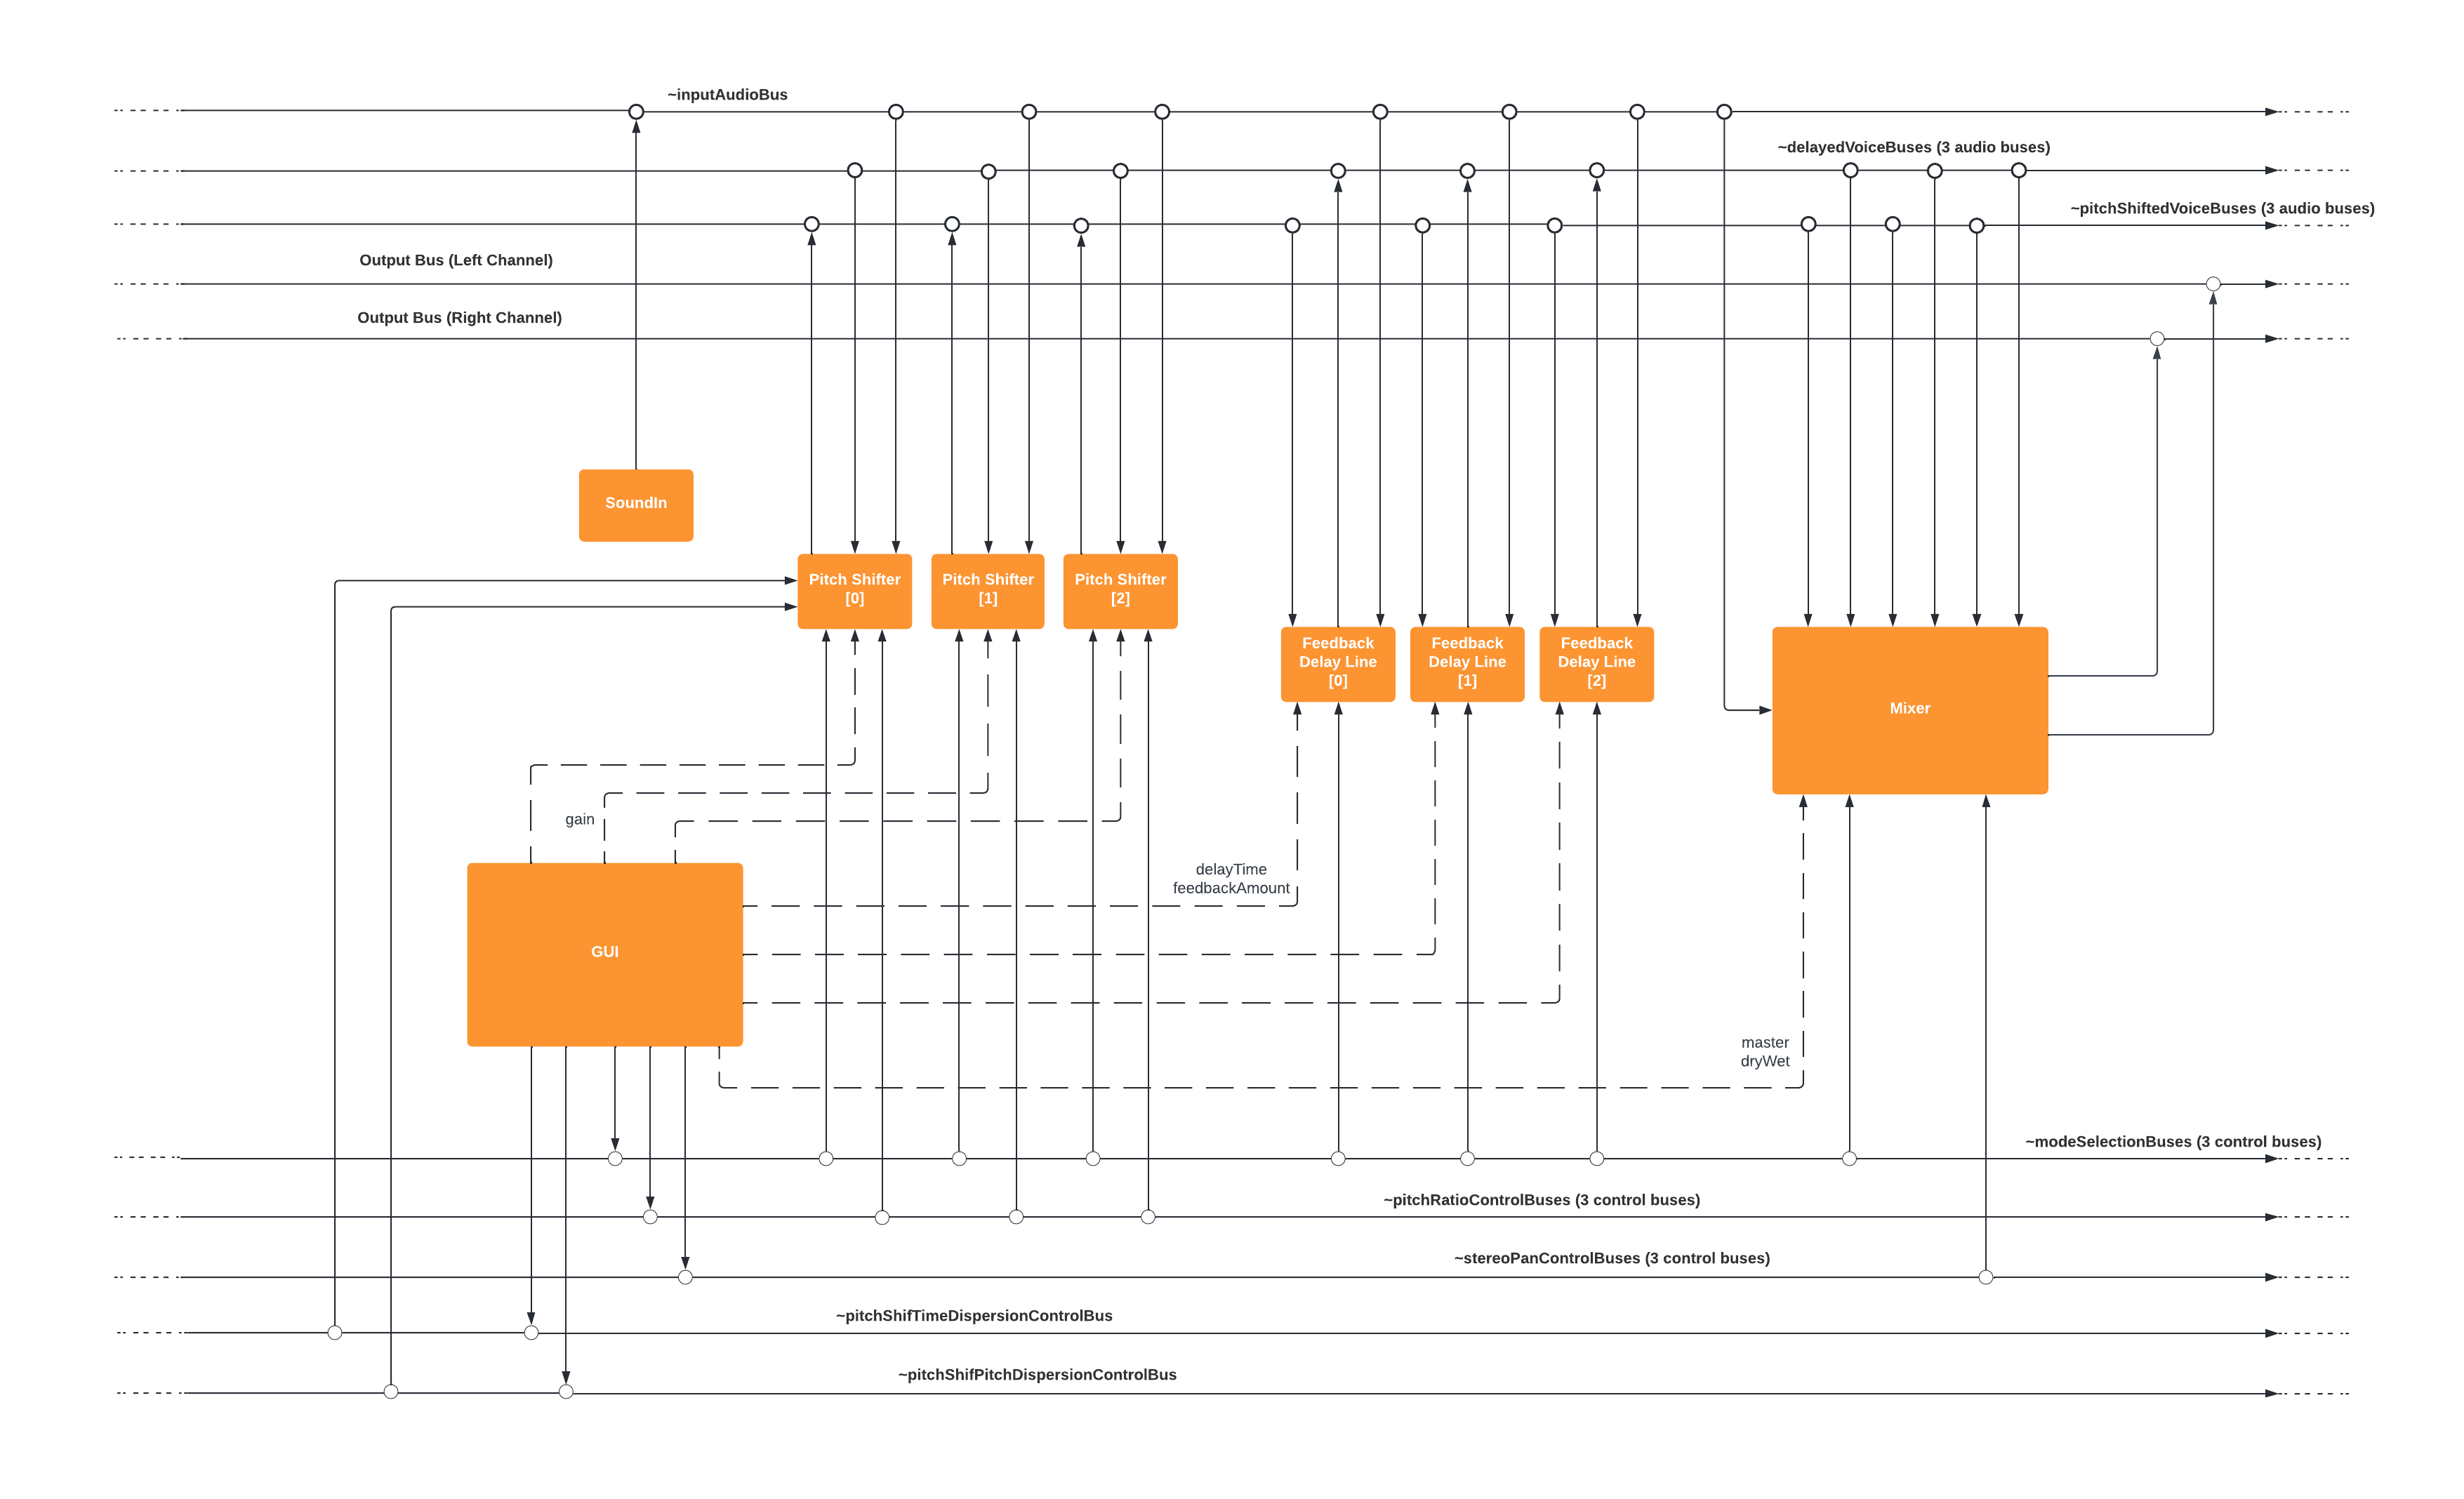
\includegraphics[width=1.0\textwidth]{Software_Architecture.png}
    \caption{Diagram of the overall architecture}
\end{figure}

\subsection{Audio Processing Block}

The audio processing chain consists of four SynthDefs: \textbf{“soundIn”}, \textbf{“pitchShifter”}, \textbf{“feedbackDelayLine”} and \textbf{“mixer”}, whose complete UGenGraphs are available on our \href{http://www.latex-tutorial.com}{Github repository} \\
\\The only goal of \textbf{“soundIn”} is to capture the input from an external device, which could be an instrument such as a guitar or a microphone, maybe routed through an external sound card. The output is then written on \textbf{\textit{$\sim$inputAudioBus}}.

The \textbf{“pitchShifter”} SynthDef takes the input from \textbf{\textit{$\sim$inputAudioBus}} and  \textbf{\textit{$\sim$delayedVoiceBuses}} and shifts it of a specified amount of semitones controlled by the GUI with the pitchRatio control, routed by \textbf{\textit{$\sim$pitchRatioControlBuses}}, which is an array of 3 buses.  The delay mode for each voice is selected thanks to the \textbf{\textit{$\sim$modeSelectionBuses}}. The goal of this block is to implement the pitch-shift, using SuperCollider’s function PitchShift, which parameters were carefully chosen to obtain a sound that would satisfy our tastes. Experimenting both with a microphone and a guitar routed through an audio interface, we found out that the optimal window size for a sound as natural as possible, was between 0.06 ms and 0.09 ms. It’s notable that we also selected a time dispersion equal to the window size, in order to keep the characteristic effect of granular pitch-shifters, such as the pitch PitchShift provided in SuperCollider. The output of \textbf{\textit{“pitchShifter”}} is then sent to \textbf{\textit{$\sim$pitchShiftedVoiceBuses}}, an array composed of three buses.

\begin{figure}[H]   
  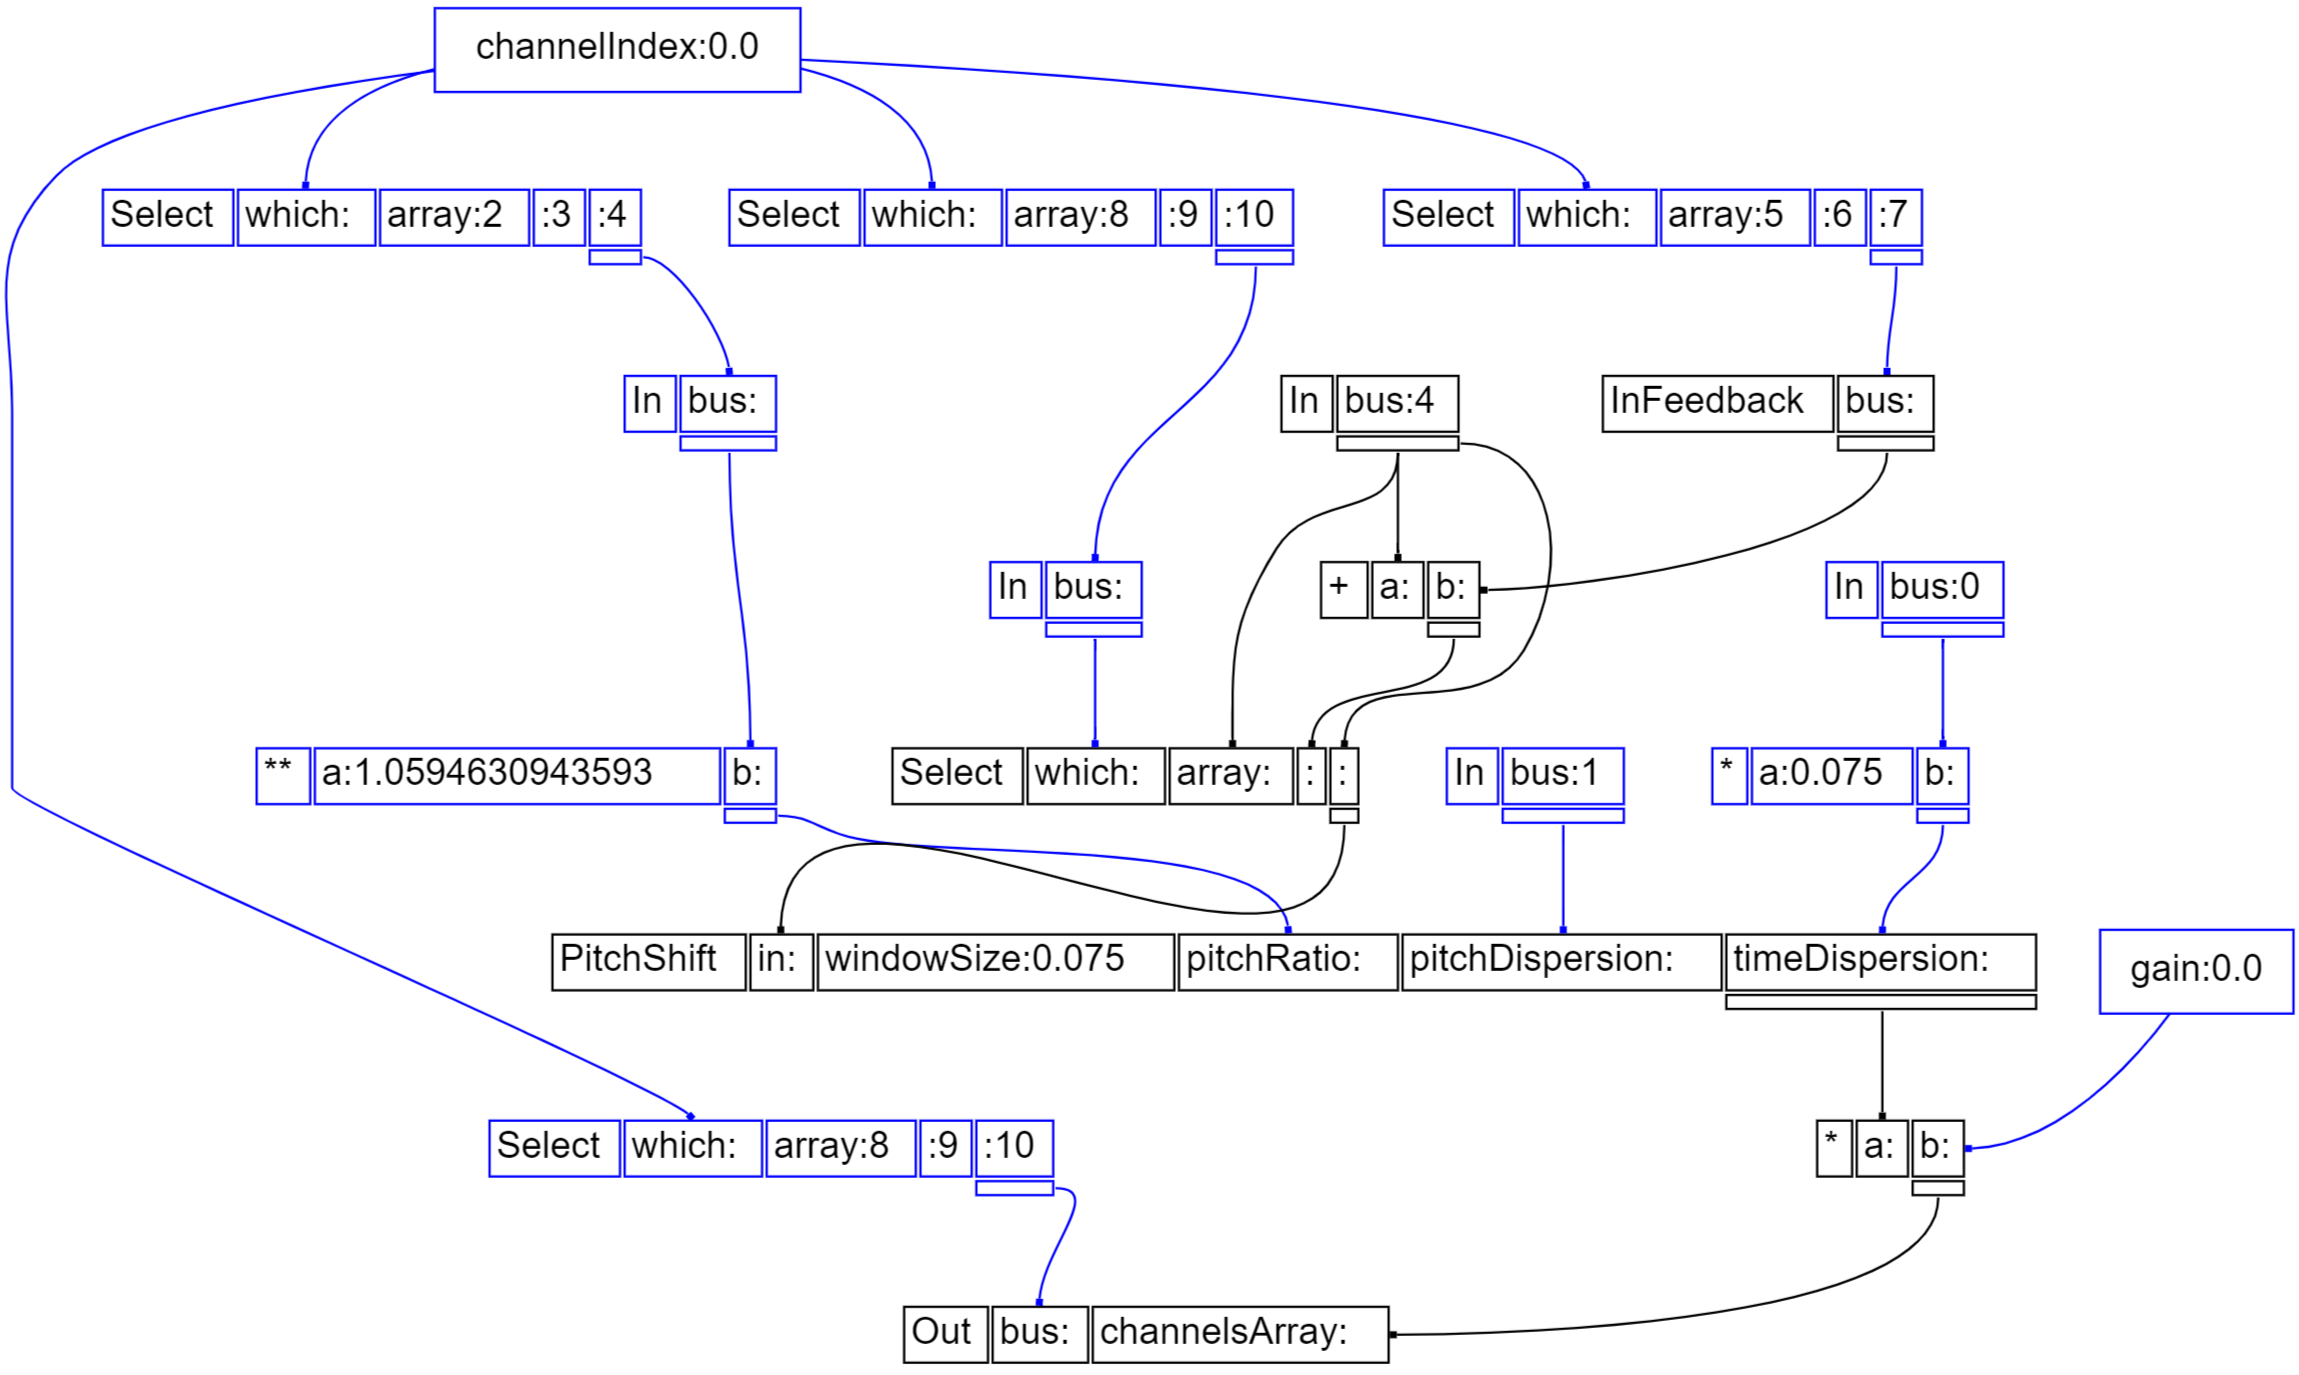
\includegraphics[width=1
  \textwidth]{UGensPitchShifter.png}
  \centering
\caption{UGens diagram of the Pitch Shifter.}
\end{figure}

The \textbf{“feedbackDelayLine”} SynthDef takes the input from the buses \textbf{\textit{$\sim$inputAudioBus}} and the\\ \textbf{\textit{$\sim$pitchShiftedVoiceBuses}}. Its goal is to apply one of the three implemented delay modes to the signal. We created a standard delay, that we identify with the name Normal, a delay that pitch-shifts the signal each iteration, called \textbf{Pitch Feedback} delay and  lastly the \textbf{Cross Feedback delay}, which draws the signal from the pitch-shifted voices of other channels. The mode is selected through the GUI using the \textbf{\textit{$\sim$modeSelectionBuses}}.

\begin{figure}[H]
\centering
    \hspace*{-20mm}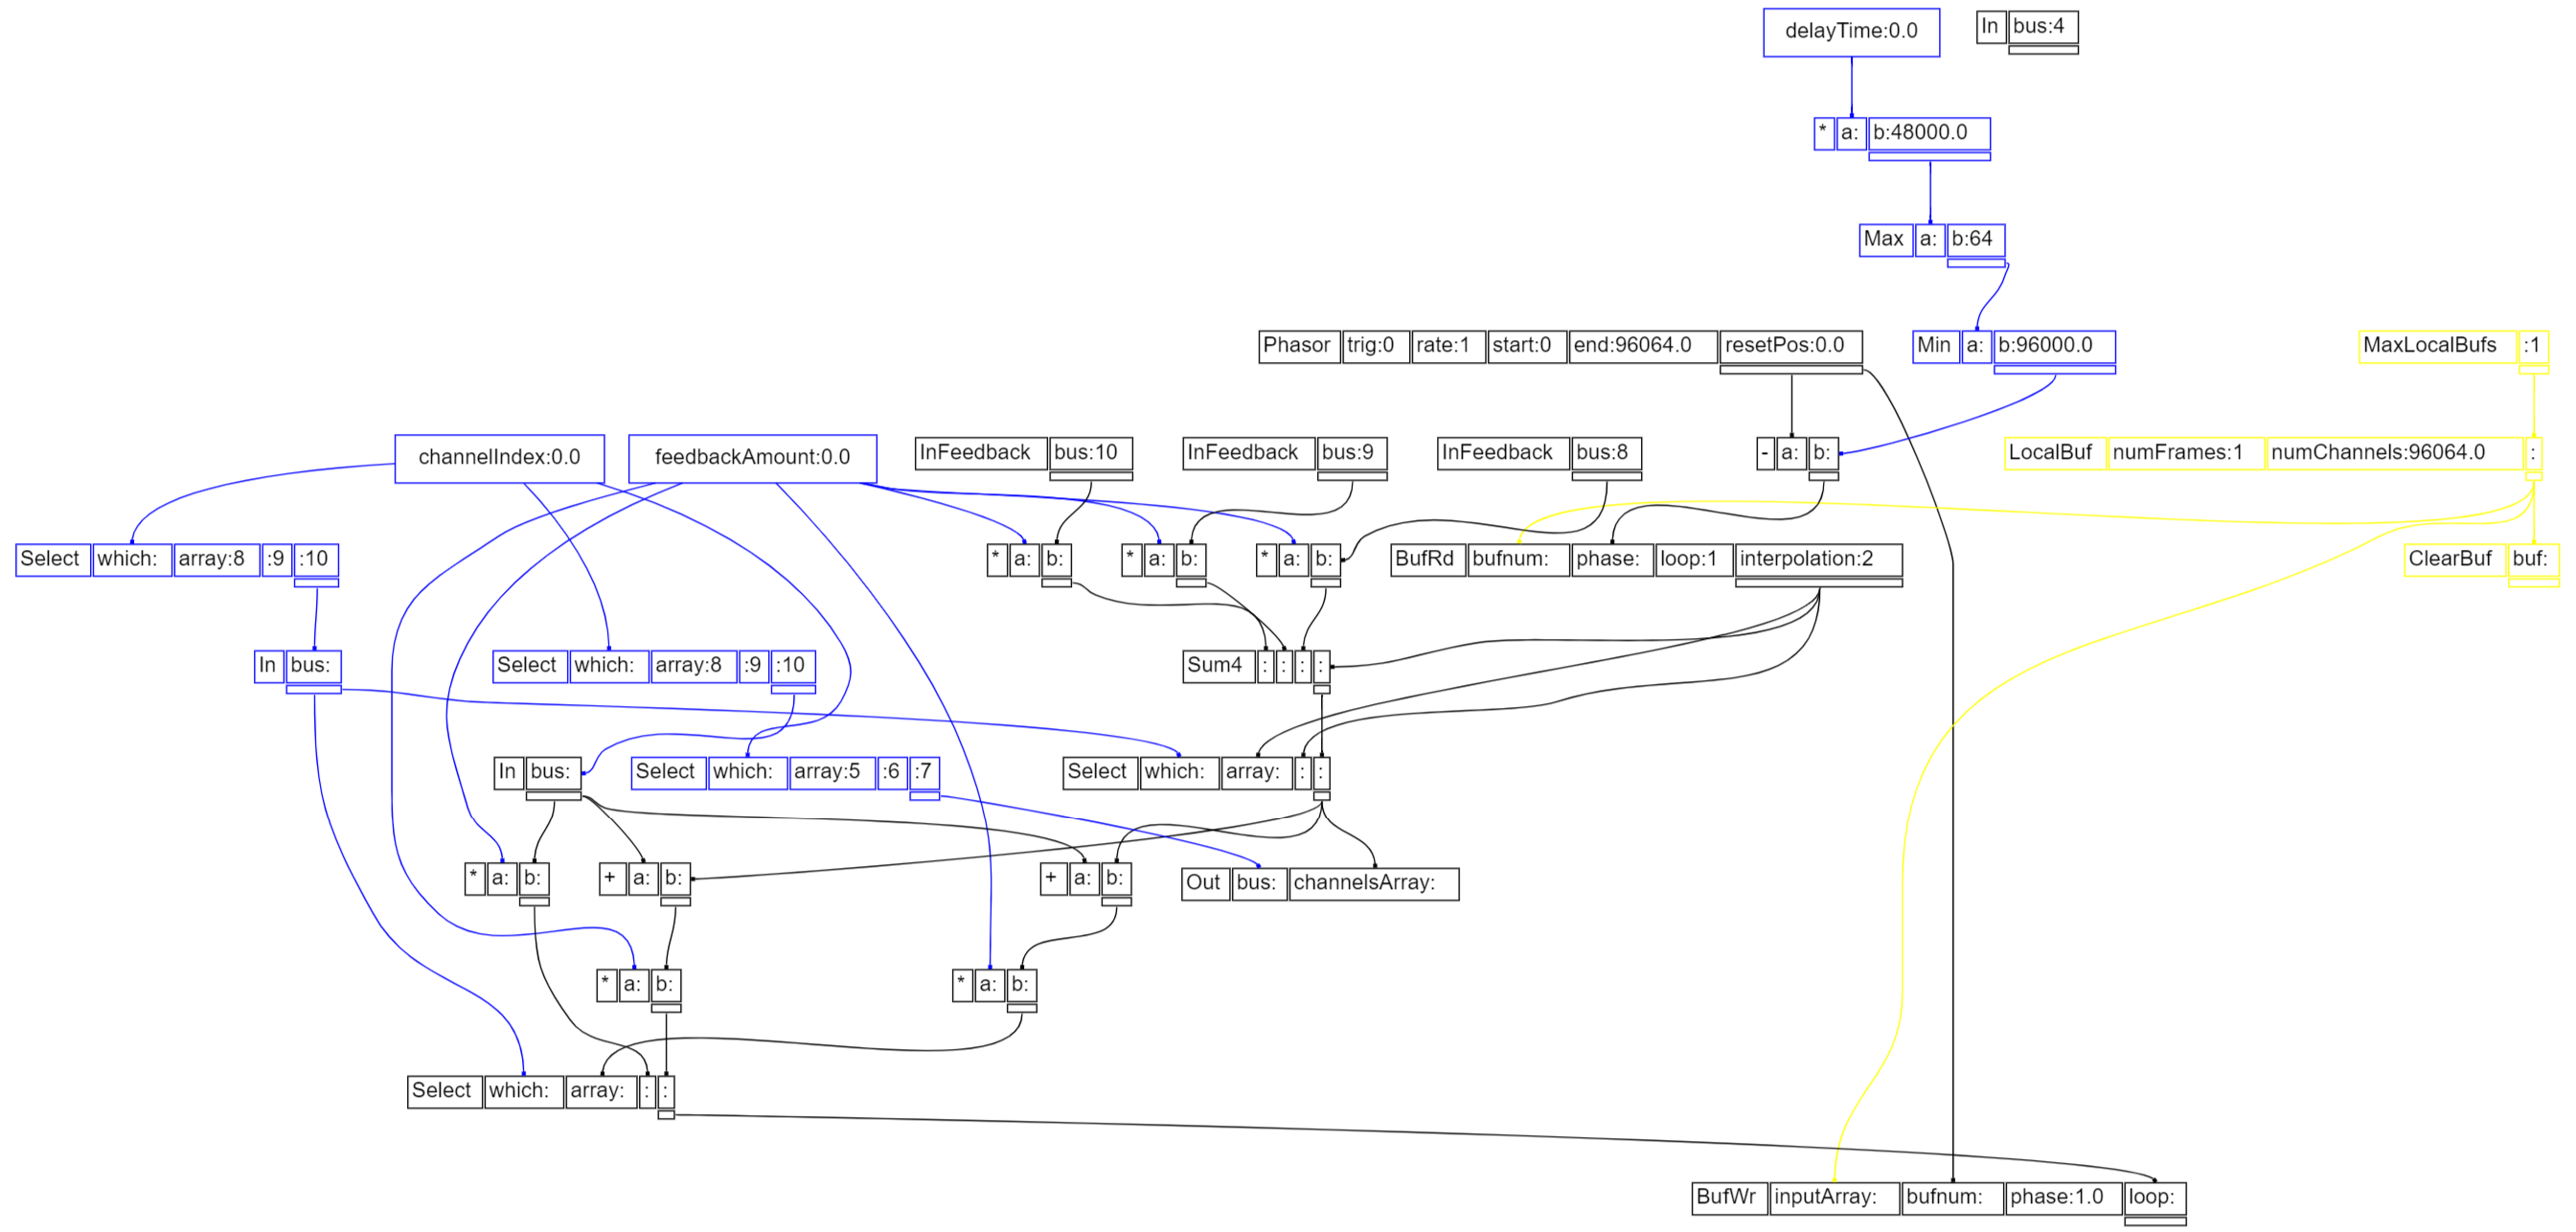
\includegraphics[width=1.2\textwidth]{UGensFeedback.png}
    \caption{UGens diagram of the Feedback Delay Line.}
\end{figure}


\subsection{Normal Delay}
The first mode we implemented acts as the most classic of delays: any input signal is fed to the \textbf{"FeedbackDelayLine"}, delayed and attenuated or boosted by a controllable factor and then fed to \\ \textbf{Feedback Delay} Line again, recursively. The result is finally reproduced, along with the original signal, resembling an echo-like effect.
\\The actual logical flow is displayed below in the 2.1 diagram. Once a signal is loaded on the input bus, the \textbf{“pitchShifter”} performs the pitch change and writes on the corresponding audio bus. Note that it only writes on a single channel of \textbf{\textit{$\sim$pitchShiftedVoiceBuses}}, choosing the one corresponding to the correct voice channel. \textbf{Feedback Delay Line} then reads from said bus, also applying a gain controlled by the $feedbackAmount$ variable. Inside this block is where the feedback happens: using Supercollider’s $FBnode$ function, we created a feedback node, which actually delays the signal by the controllable variable \textbf{delayTime}. \\The recursion is finally obtained, writing on the correct element of \textbf{\textit{$\sim$delayedVoiceBuses}}  and feeding it in the \textbf{Feedback Delay Line} again. Lastly, In order to reproduce the effect, the \textbf{Mixer} reads from \textbf{\textit{$\sim$pitchShiftedVoiceBuses}} and \textbf{\textit{$\sim$delayedVoiceBuses}}, mixing them together with the original input.

\begin{figure}[H]
\centering
  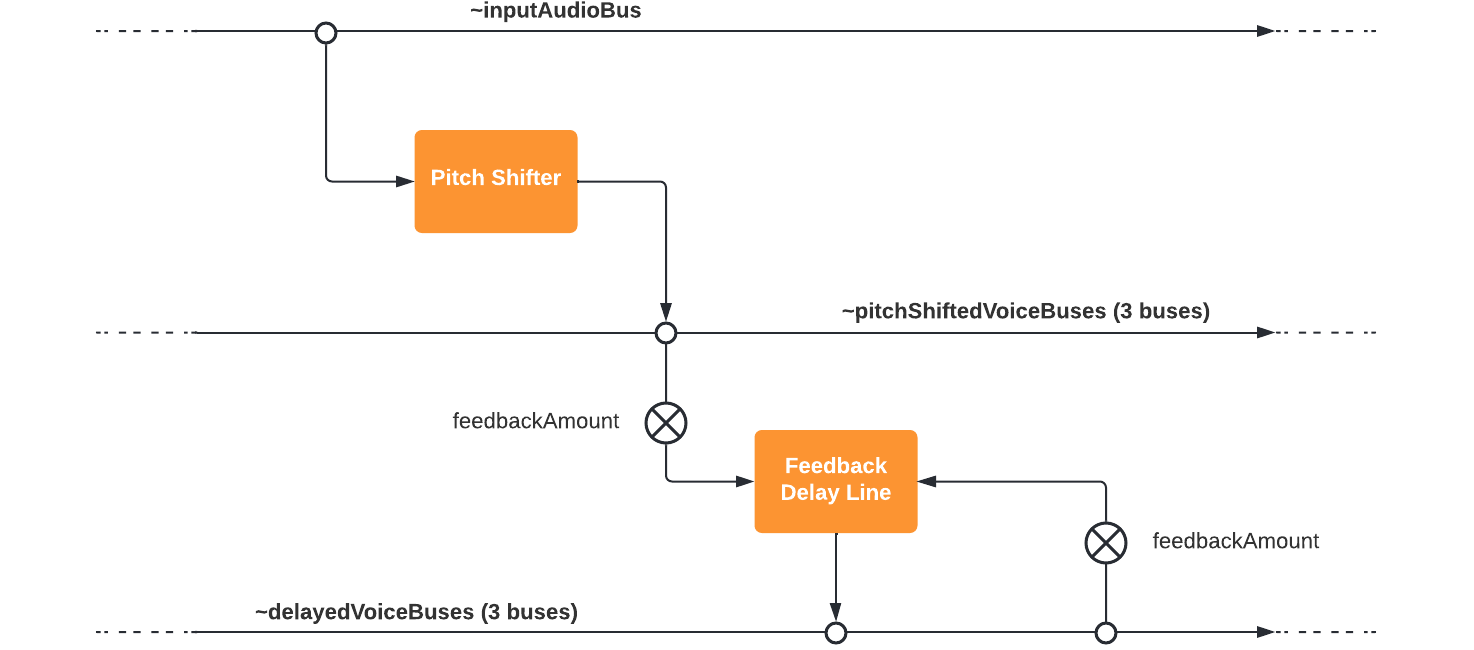
\includegraphics[width=0.6\textwidth]{Normal_Feedback.png}
    \caption{Diagram of the Normal delay.}
\end{figure}

\subsection{Pitch Shifted Delay}
The second mode is basically the classic echo, but with a twist: each recursive iteration does not simply delay the signal, but also applies the pitch-shift again. The result is an echo, which pitch increases (or decreases) each iteration by the amount shown in the Pitch Ratio parameter of the same voice.
\\As displayed in the \textit{2.2 diagram}, the procedure is quite similar to the \textbf{Normal delay} one, the only difference being the \textbf{Pitch Shifter} reading from \textbf{\textit{$\sim$delayedVoiceBuses}} instead of the \textbf{Feedback Delay Line}. This means that the recursion loop this time also includes the \textbf{Pitch Shifter}, resulting in the already mentioned iterative pitch-shifts. In this case the mixer, which is not shown in the diagram for tidiness, only reads from \textbf{\textit{$\sim$pitchShiftedVoiceBuses}} and puts it together with the dry signal to obtain the final result.

\begin{figure}[H]
\centering
  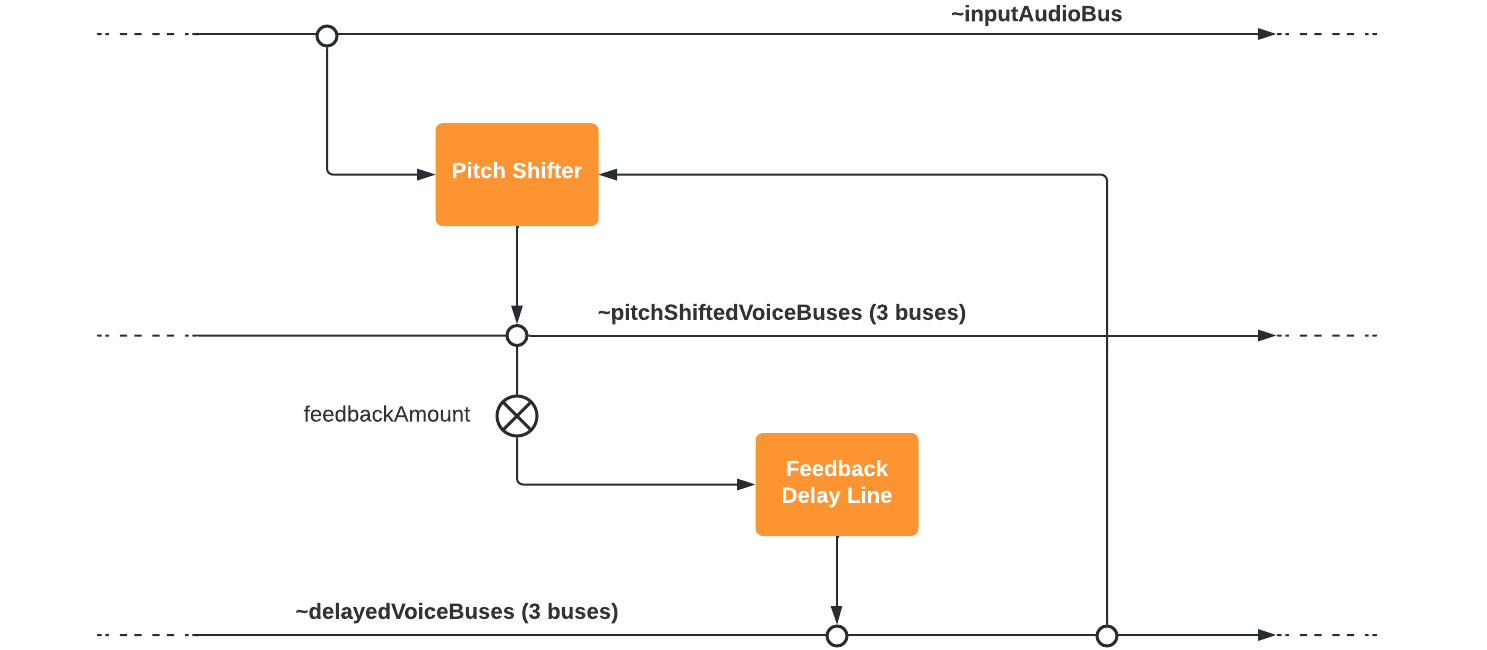
\includegraphics[width=0.6\textwidth]{Pitch_Feedback.png}
    \caption{Diagram of the Pitch Shifted Delay.}
\end{figure}

\subsection{Cross Feedback Delay}
The third mode is the most experimental and complex out of the three. It was designed to generate an effect that would bounce between the two output channels, exploiting Pan usage, but adding the interchange of signals between the channels made the creation of even more whimsical sounds possible.
\\Although the \textit{2.3 diagram} is a bit more complex than the others, the basic structure still resembles the Normal Delay. We can see that the recursion happens in the same way and that the feedback amount factor is still used in the same way. The main difference is that in this case the \textbf{Pitch Shifters} read from two buses instead of one, picking them to have a different index than its one. Finally the \textbf{Mixer} reads from both \textbf{\textit{$\sim$pitchShiftedVoiceBuses}} and \textbf{\textit{$\sim$delayedVoiceBuses}}, adds them back together, obtaining the final result.

\begin{figure}[H]
\centering
  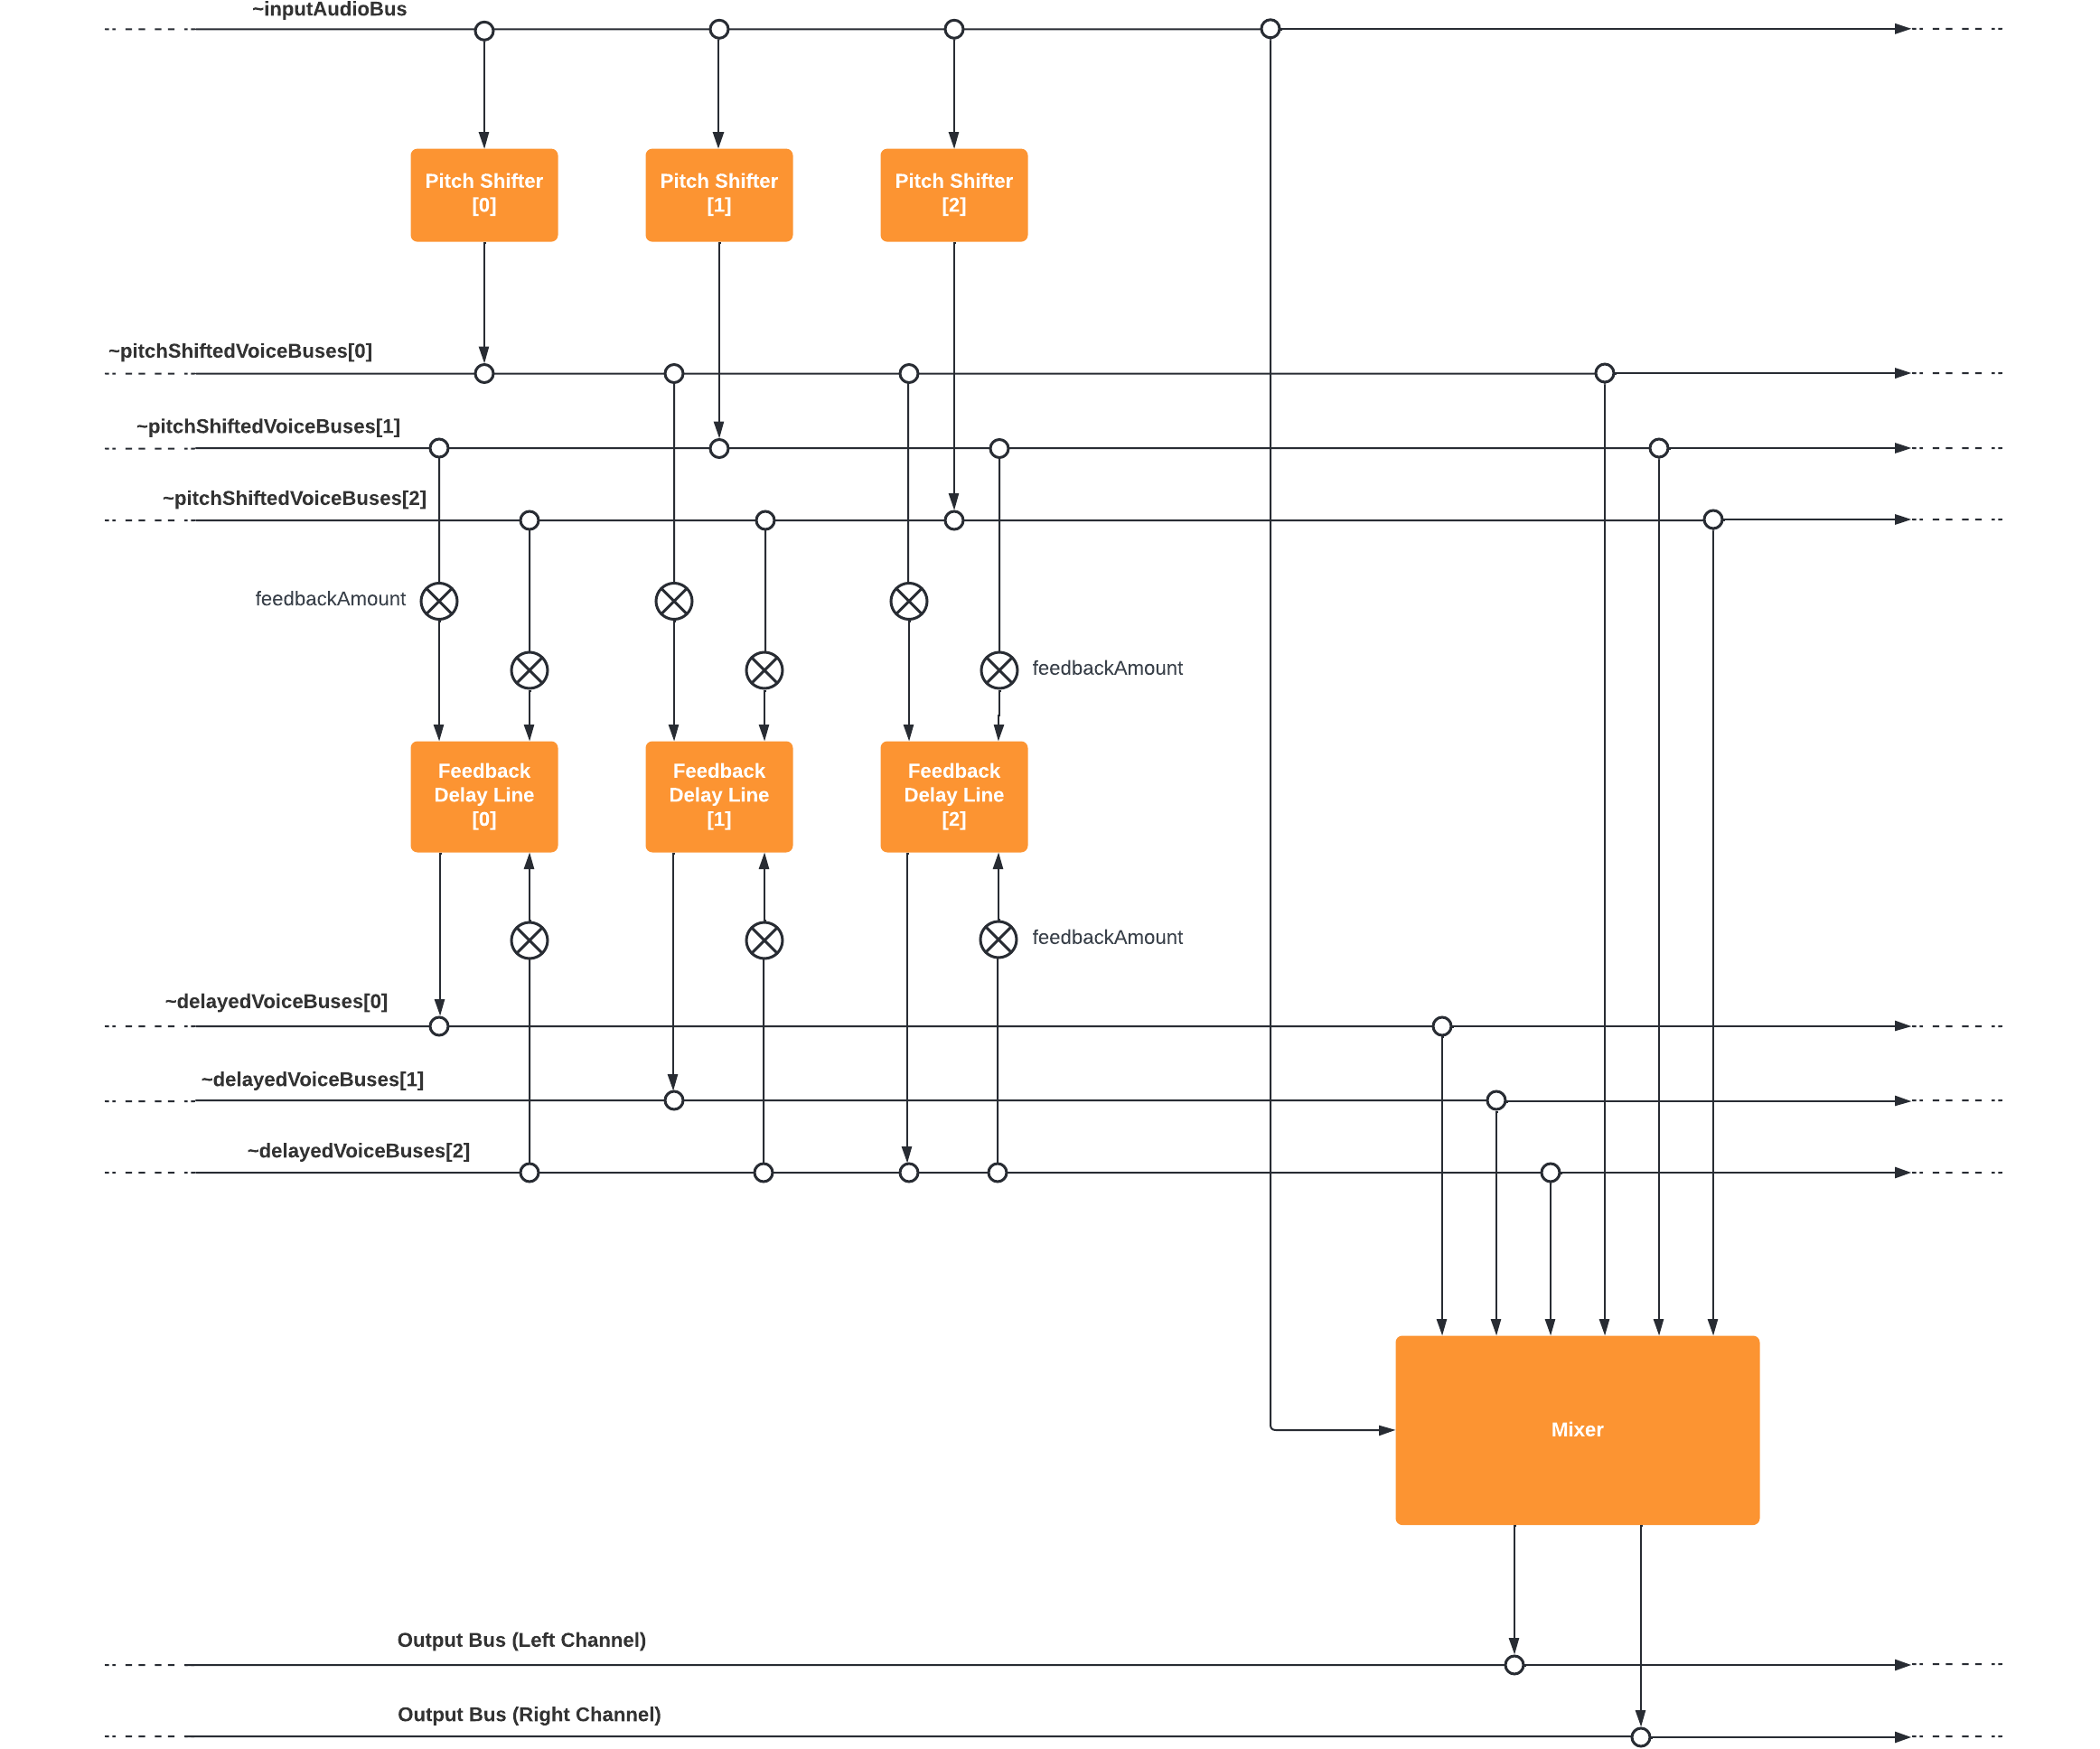
\includegraphics[width=0.6\textwidth]{Cross_Feedback.png}
    \caption{Diagram of the Cross Feedback Delay.}
\end{figure}

\subsection{Graphical User Interface}
The graphical user interface (GUI) of the software provides the musician with three main sections:
\textbf{Master}, \textbf{Pitch Shifter} and  \textbf{Voices section}.

\begin{figure}[H]
    \centering
    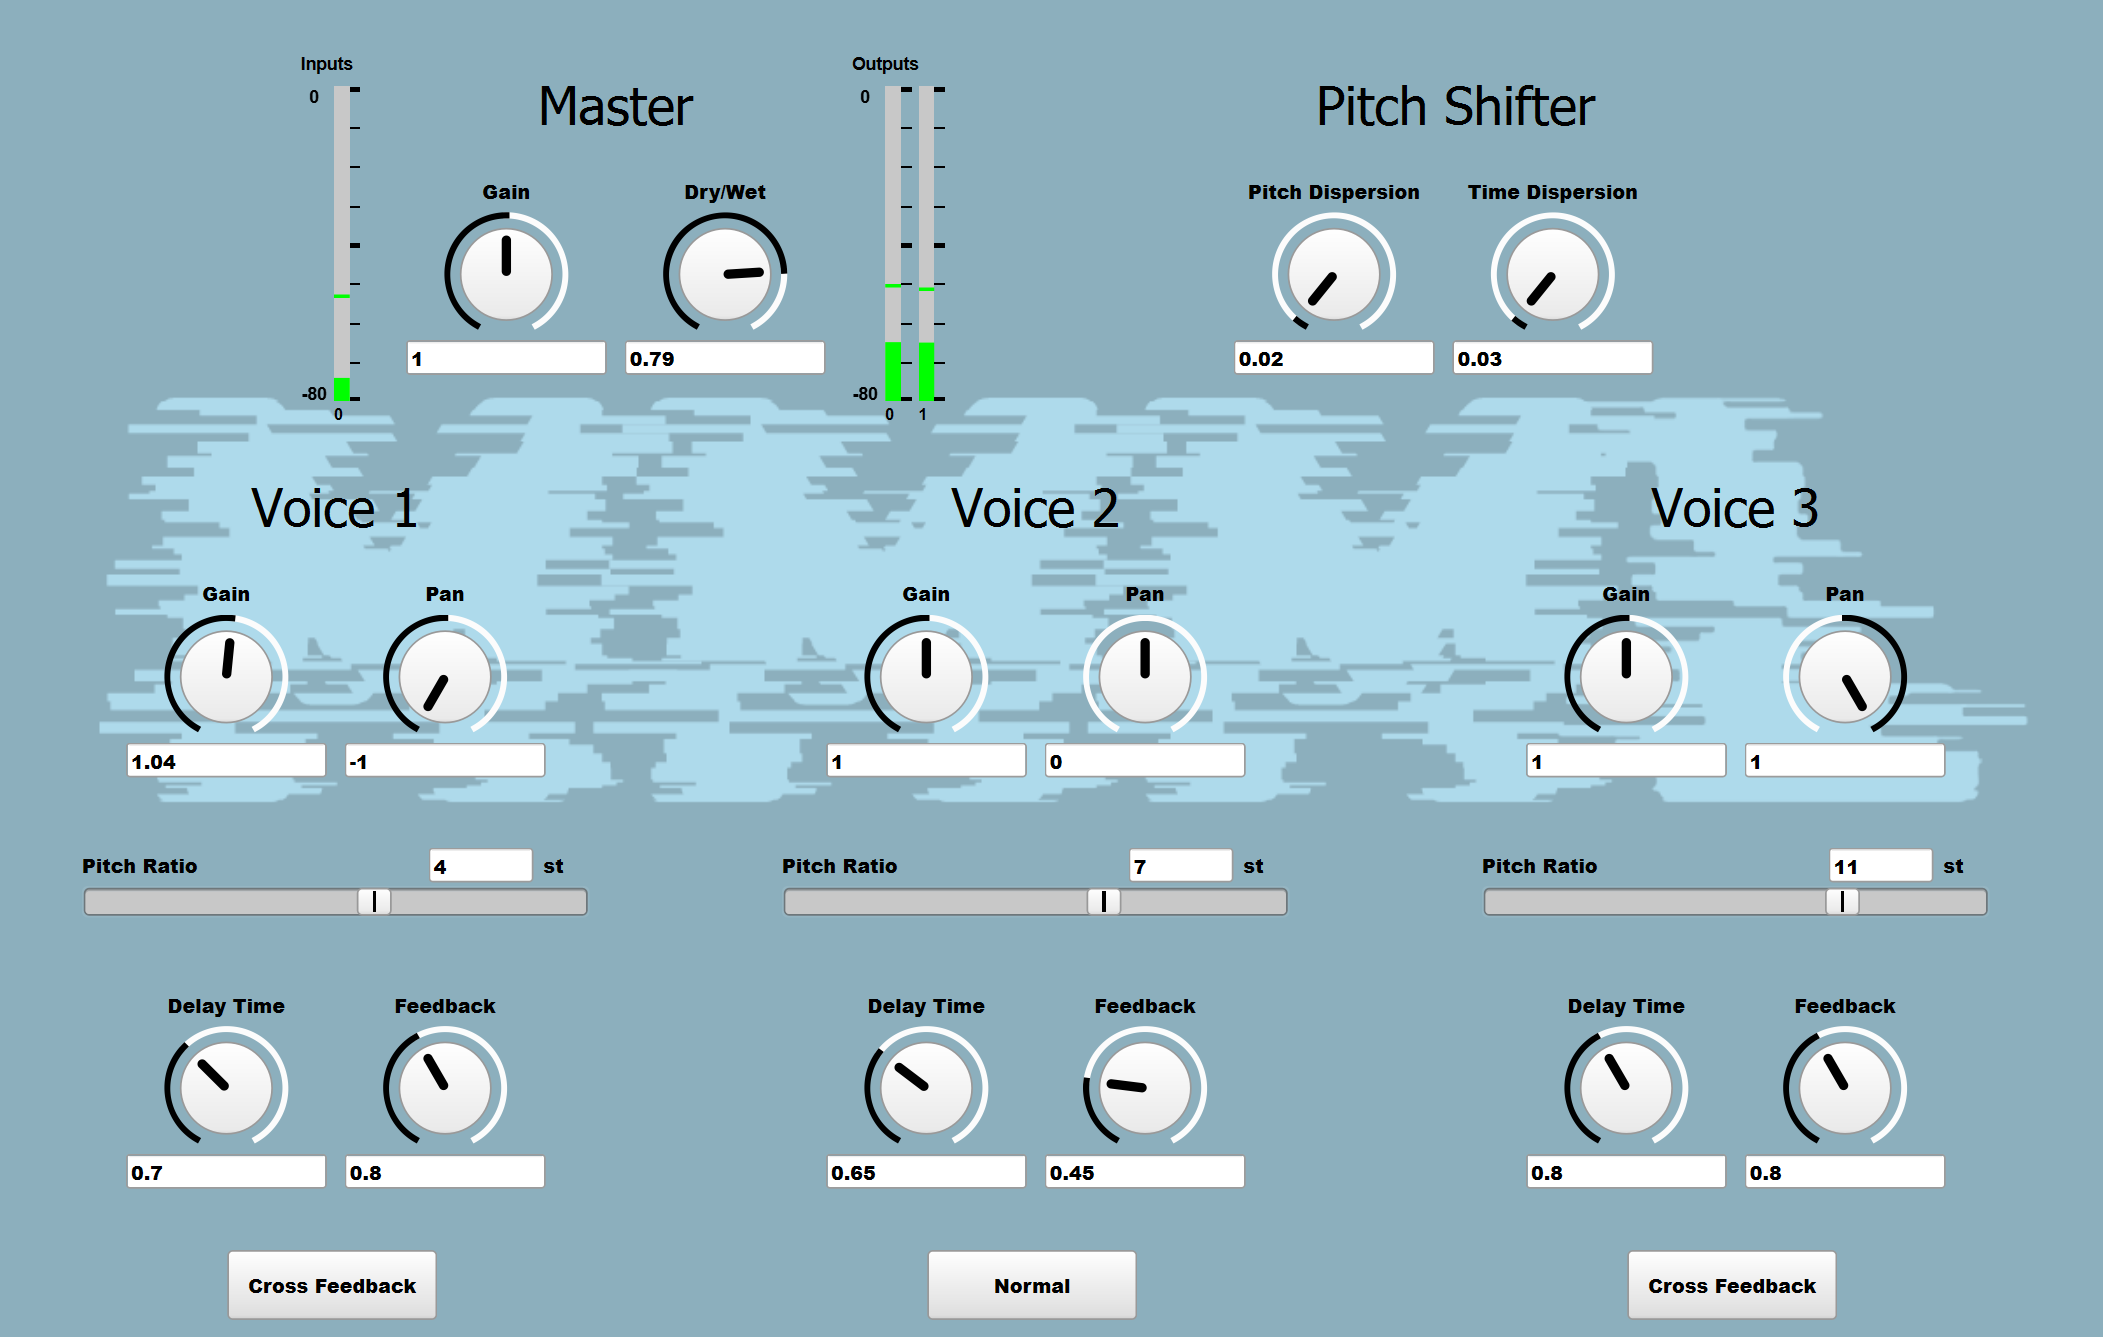
\includegraphics[width=0.7\textwidth]{GuiOverview.png}
    \caption{Graphical User Interface of the software}
\end{figure}

\begin{wrapfigure}{l}{0.4\textwidth}
    {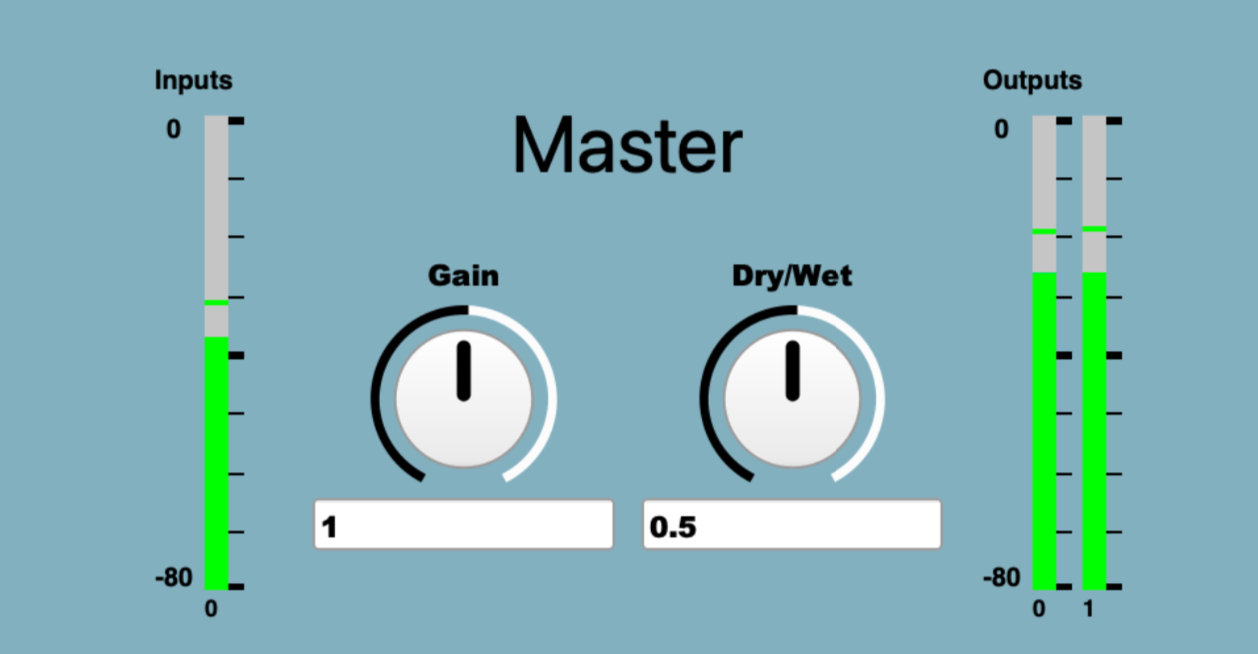
\includegraphics[width=5.5cm]{GuiMaster.png}}\par
    \caption{GUI - Master section.}
    \vspace{3mm}
    {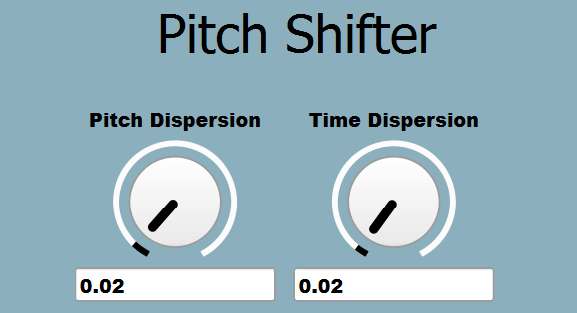
\includegraphics[width=5.5cm]{GuiPitchShifter.png}}\par
    \caption{GUI - Pitch Shifter section.}
    {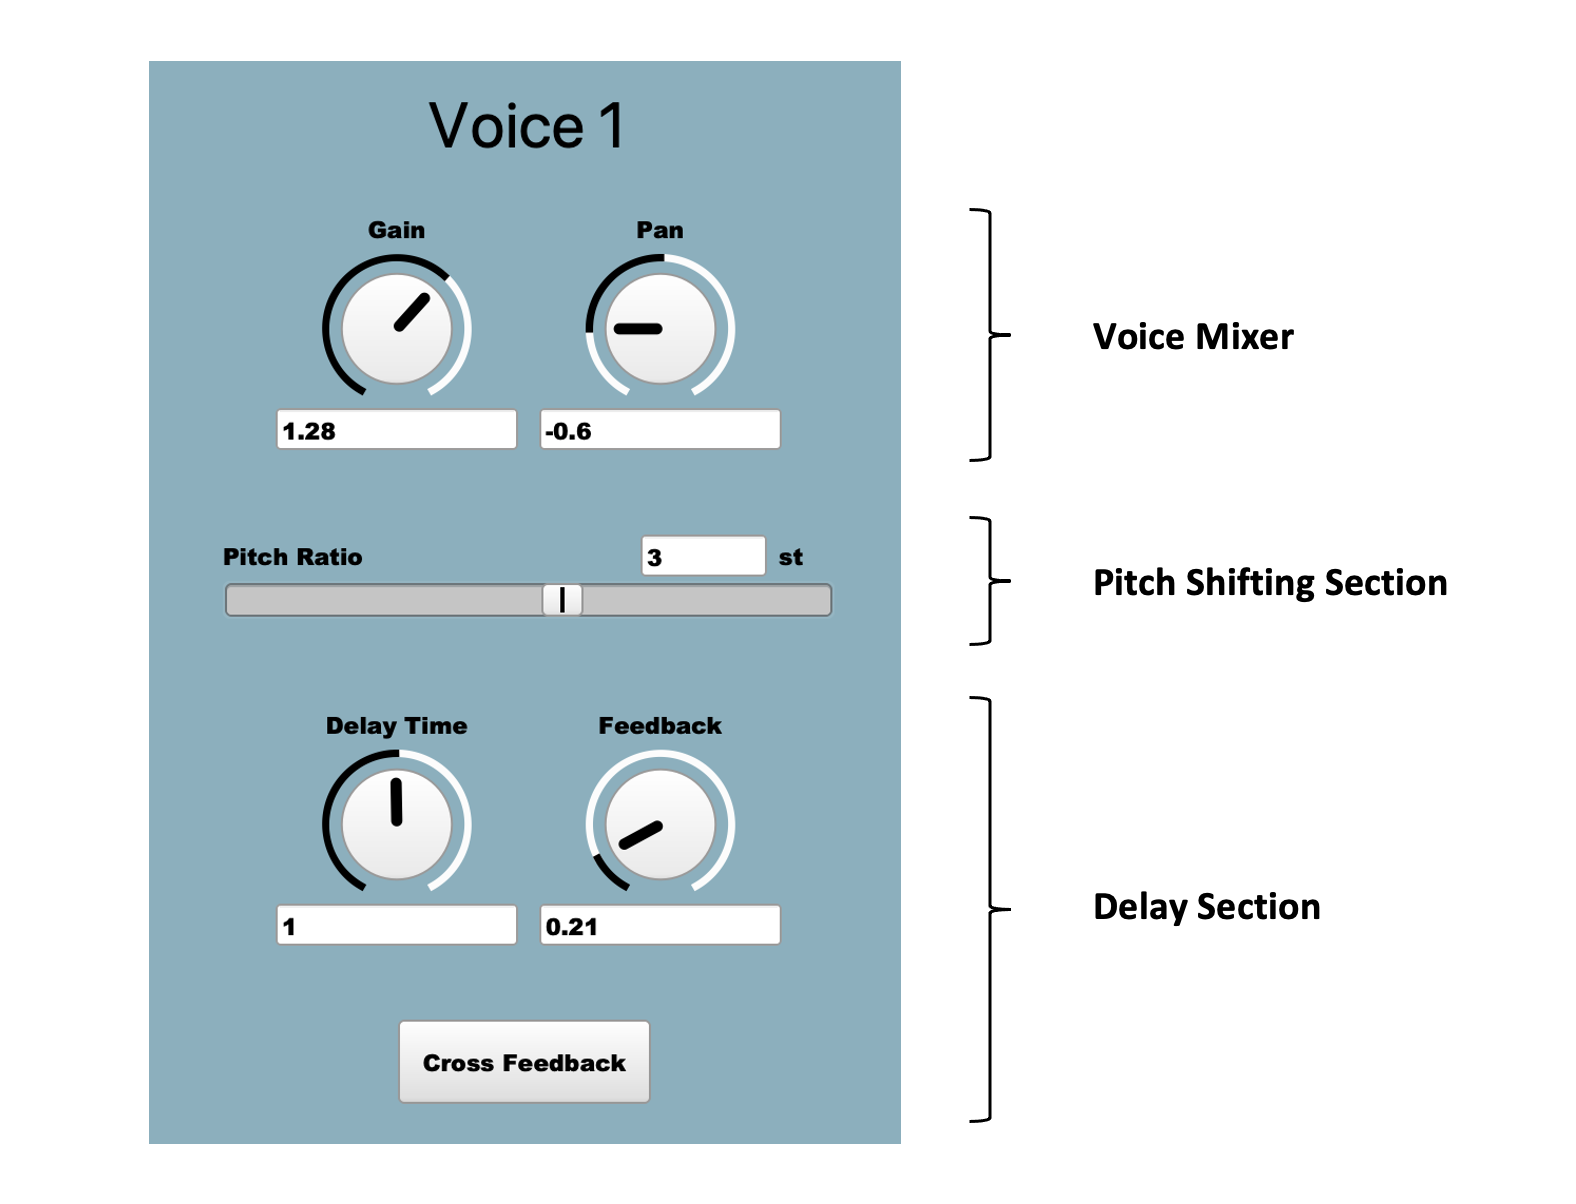
\includegraphics[width=7cm]{GuiSingleVoiceSections.png}}\par
    \caption{GUI - Single Voice}\vspace{-28mm}
\end{wrapfigure}

At the top left, the \textbf{master} section offers two knobs \textit{(Figure 7)} through which the musician can control the gain of the final output and dry/wet balance between the clean input signal and the pitched voices. In addition to this, two meters related to input and output signals respectively are rendered so that the user is aware of potential distortion.

At the top right, the \textbf{Pitch Shifter} \textit{(Figure 8)} control section allows the user to set Pitch Dispersion and Time Dispersion values. As said before, these parameters are shared between all three pitch-shifter instances which process the different voices individually.

Then, the voices section is divided into three panels, one for each voice generated by the harmonizer. Every panel is in turn composed of three subsections:
\begin{itemize}
  \item \textbf{Voice Mixer} sets the gain and stereo pan of the corresponding voice.
  \item \textbf{Pitch Shifting} section shows a pitch ratio slider which makes it possible to set the target pitch of the voice by selecting the pitch ratio value given in the number of semitones above or below the original pitch.
  \item \textbf{Delay Section} provides control over some parameters of delay effect to be applied on the single voice. In fact, one can set the delay time in milliseconds and the feedback amount. Moreover, a button at the bottom center allows the artist to choose between three different feedback setups (implementation described within the previous section of the report): Normal, Pitch Feedback and Cross Feedback.
  \vspace{10mm}
\end{itemize}

{
\section{Conclusions}
\subsection{Results}
Summing up our work, we produced a working harmonizer that allows manipulating all three voices’ gain, pitch-shift and pan, as well as global volume and wet controls. On top of that, we added three different delays that allow both more traditional effects and more experimental ones.}
\\The first challenge we faced was setting up the pitch-shifting block, which is the core of our harmonizer. 
\\Moreover, we really found the part about delay modes interesting and, in particular, we appreciated the part of designing increasingly complex models that we would use to obtain them.
\\Besides those aspects, what we are most satisfied with is for sure the architecture we achieved. Thanks to a modular structure and extensive usage of buses we were able to generate all harmonizer’s voices iteratively, achieving a scalable and sustainable code, making any future changes easier. For example, even major changes such as increasing the number of available voices would be possible just by adding iterations to the loop, adjusting bus dimensions and elements position in the graphic user interface.



\subsection{Future Improvements}
Even if we are quite satisfied with our final result, due to limited time, we couldn’t implement all the ideas that we had. Between the ideas in line we thought  of creating an harmonic mode selector, that would allow a scale selection and we indeed started creating a pitch follower, that didn’t find usage in our final version. Beside that, we had some ideas for more complex graphics and to apply a reverb to to the final mixed signal, but had them momentarily set aside.

\end{document}